% !TeX spellcheck = da_DK
\input{../common/preamble.tex}

\title{Drift}
\author{Silas Bergishagen Christiansen \& Redigeret af Kristian Anton Hedegaard}
\date{\formatdate{16}{2}{2026} \& Redigeret \formatdate{6}{5}{2026}}

\begin{document}

\maketitle

\section{Introduktion}

Som Drift i Fredagscaféen har man ansvaret for vedligehold af baren og især fadølsanlægget. Det indeholder også at tage fat i bygningsdrift i tilfælde af AU's ejendom, så som stole, borde, toiletter, skulle gå i stykker eller på anden måde tage skade under en barvagt.

Få styr på hvor forskellige ting kan findes, og hvad der kunne opstå af mangler. F.eks. kan værktøj findes i \textit{træburet}, og reservedele til fadølsanlægget \textit{bag gitteret} (mindre reservedele i den røde kasse). Opstår der tvivl om hvordan noget gøres eller repareres, så spørg mere erfarne bestyrelsesmedlemmer til råds. Søgemaskiner, YouTube og LLM'er kan også hjælpe.

\subsection{Bygningsdrift}

Nat-Tech Bygningsdrift befinder sig i Hopper 040. Fornyligt har de fået et nyt system til indmelding, og den gamle mailaddressen er blevet pillet ned. Instruktioner hænger til højre for deres kontordør.

\section{Troubleshooting af fadølsanlægget}

\begin{itemize}
    \item Er fadølsanlægget sat til strøm?
    \item Er fadkoblingen monteret rigtigt?
    \item Er slangerne sat til fadkoblingen?
    \item Er fustagen tom?
    \item Er gasflasken tom?
    \item Er der tændt for gassen?
    \item Er trykket indstillet fornuftigt?
    \item Er noget synligt i stykker?
\end{itemize}

\section{Ting at være opmærksom på}

\begin{description}
    \item[Slangerne i fadølsanlægget] skal skiftes senest hvert 5. år -- det kan anbefales at være flere om det. De er sidst blevet skiftet i april 2025.
    \item[Rensningsdunkene] har en udløbsdato. De skal skiftes inden 2027.
    \item[Gasslangerne] skal være tørlagt. Dug er normalt og gør ikke noget, men hvis der er kommet væske i skal den skiftes.
    \item[Timeren til fadølsanlægget] skal den stilles igen, hvis det tages ud af stikket. Den burde dog huske tidligere ``modes''.
    \item[Industriopvaskeren] i DatKant kan give fejlkoder, typisk grundet sensorfejl. De kan normalt cleares på `C', så en pantvagt kan forsættes. Tag dog højde for om fejlen er kritisk.
    \item[Afspændingsmiddel] til industriopvaskeren er før bestilt igennem Mads fra MatKant (\email{mac@math.au.dk}), så sørger de for at sætte en ny til.
    \item[Gas grillen] har to hovedbrændere der er i udu grundet mangel på gastilførrelse. Der er enten noget i vejen med knapperne eller kablerne.
    \item[Fadølskøleren] kan ``dryppe'' grundet kondens fra kulden når det har stået tændt tilstrækkeligt længe. 
    \item Om der skal bestilles flere reservedele til anlægget. Vi har tidligere bestilt fra \url{https://holtecsolutions.dk/}, hvor vi også har en konto. Køb skal ofte igennem Kassereren først, da de har overbliv over barens økonomi og betaling. Man kan også selv lægge ud, men her er det en god ide, at få tilladelse til dette på forhånd.
\end{description}


\section{Koblinger til fadøl}
Vi har 4 slags koblinger til fadøl/fustager. Her er en oversigt over dem, og hvad de bruges til:

\subsection{S-kobling}
Vi bruger S-kobling til ALT fra Aarhus Bryghus. Det er en standard kobling, der passer til langt de fleste normale fustager på markedet (Carlsberg, Royal, Hancock, osv.). Vi bruger også S-kobling på rensedunkene, og til at tømme slangerne for vand, med blændkop/blindkobling.
\begin{figure*}[h]
    \centering
    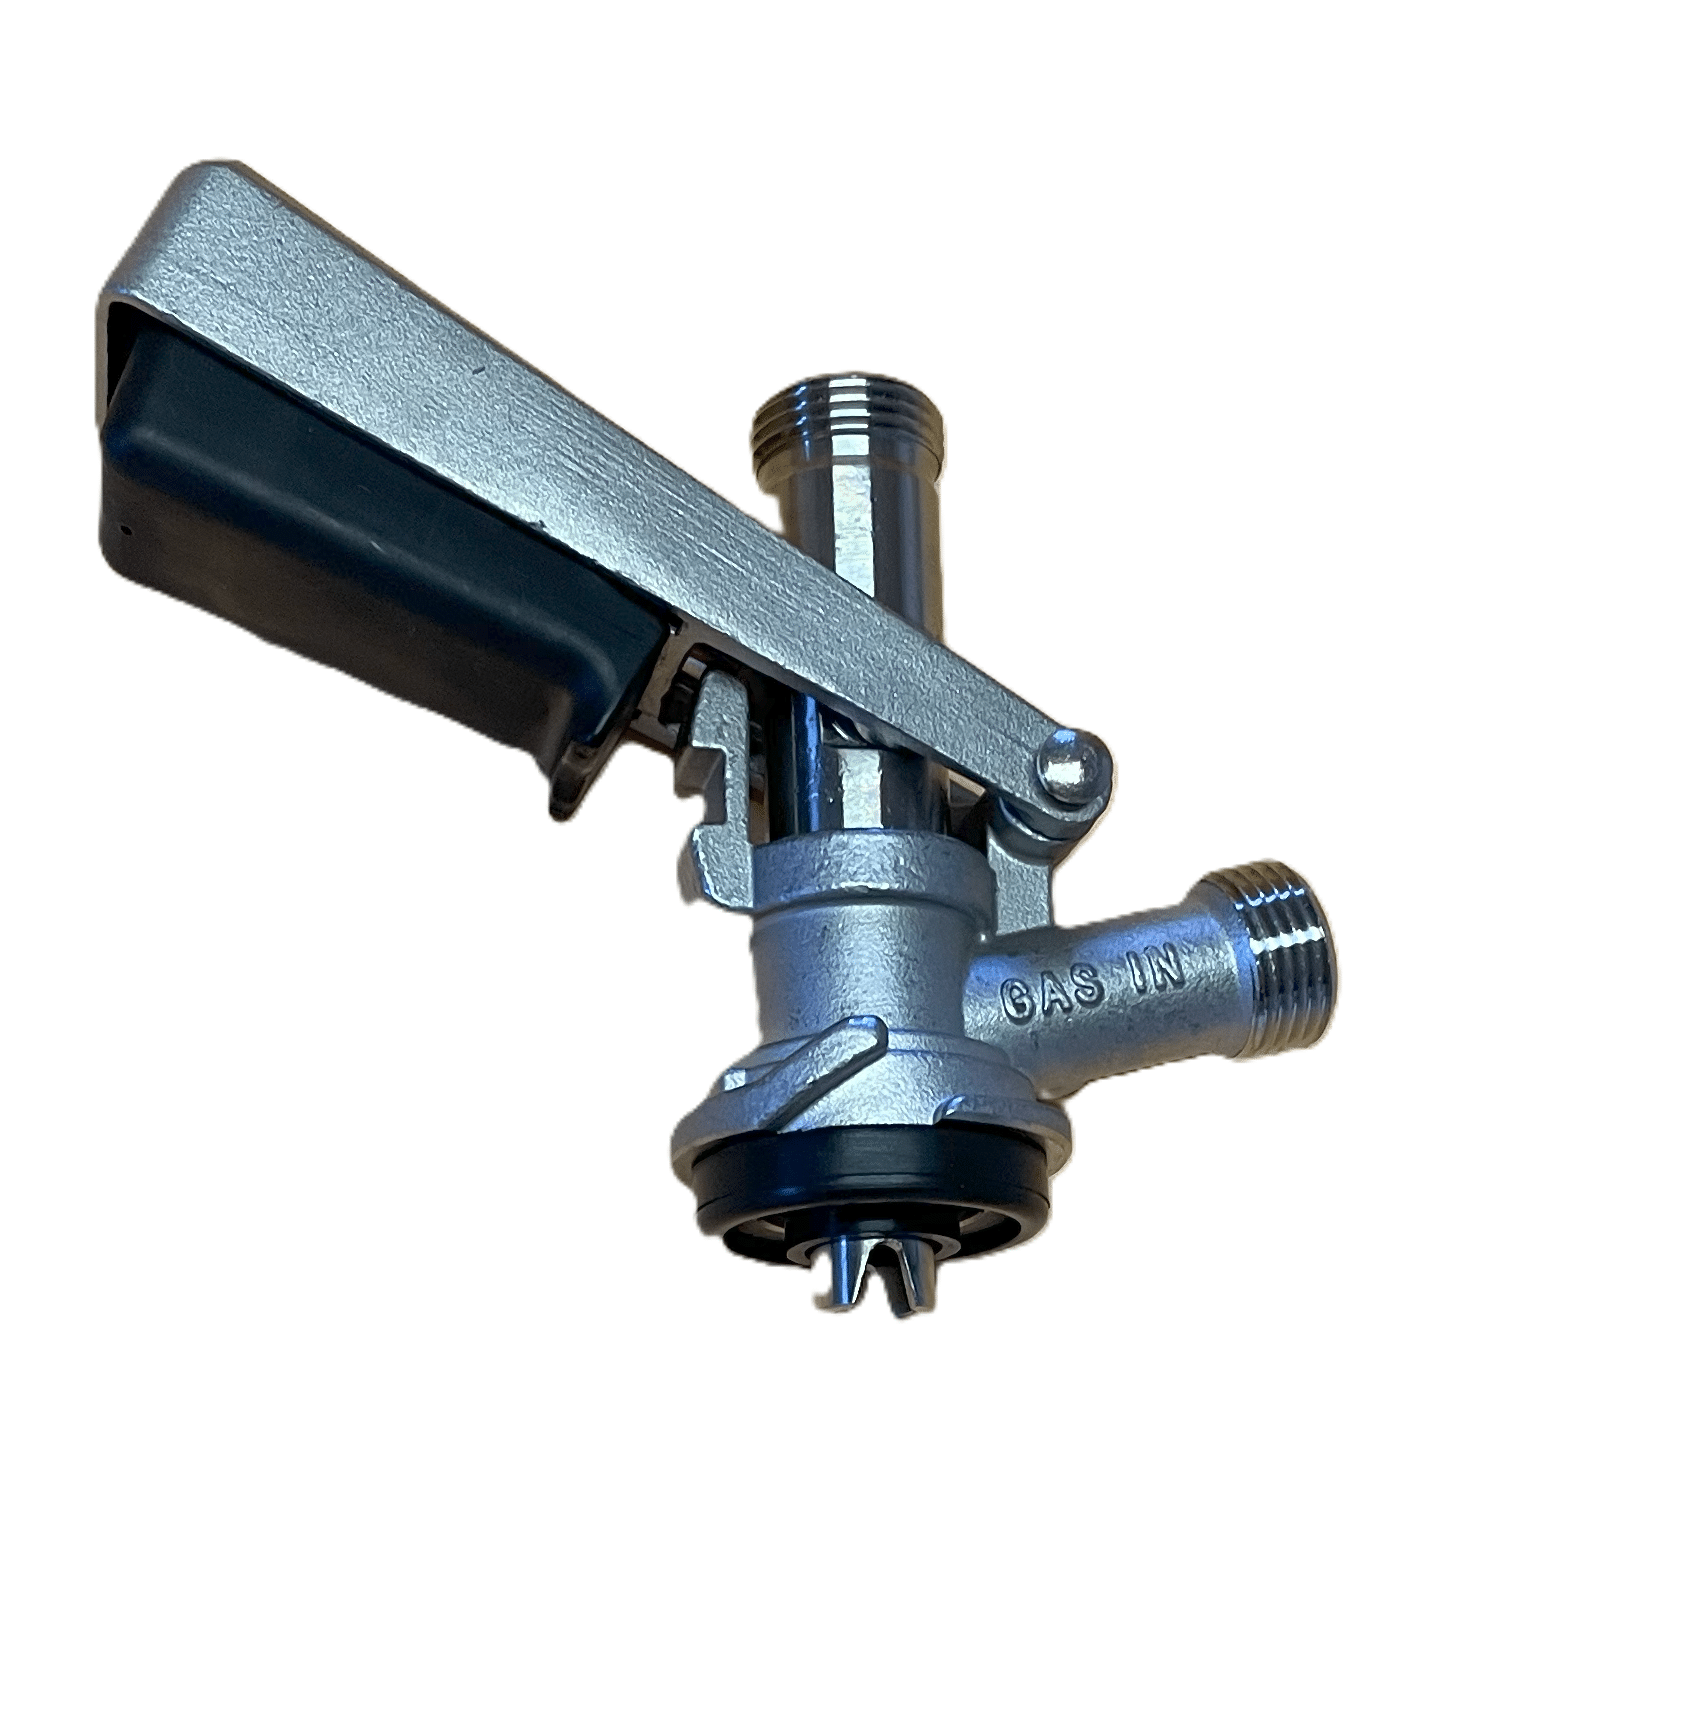
\includegraphics[width=0.5\textwidth]{S-kobling.png}
    \caption{S-kobling}
\end{figure*}

\subsection{U-kobling}
U-koblingen ligner S-koblingen, men den er bredere og rund i bunden. Den bruges til bla. Magners cider og Guinness. 
\begin{figure*}[h]
    \centering
    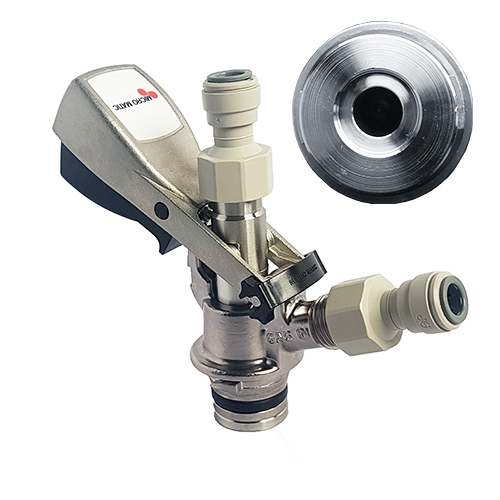
\includegraphics[width=0.5\textwidth]{U-kobling.png}
    \caption{U-kobling}
\end{figure*}

\subsection{KeyKeg-kobling}
KeyKeg-koblingen er en rund kobling, der bruges til KeyKeg fustager (Engangsfustager I plast). Vi bruger dem ofte til specialøl.
\begin{figure*}[h]
    \centering
    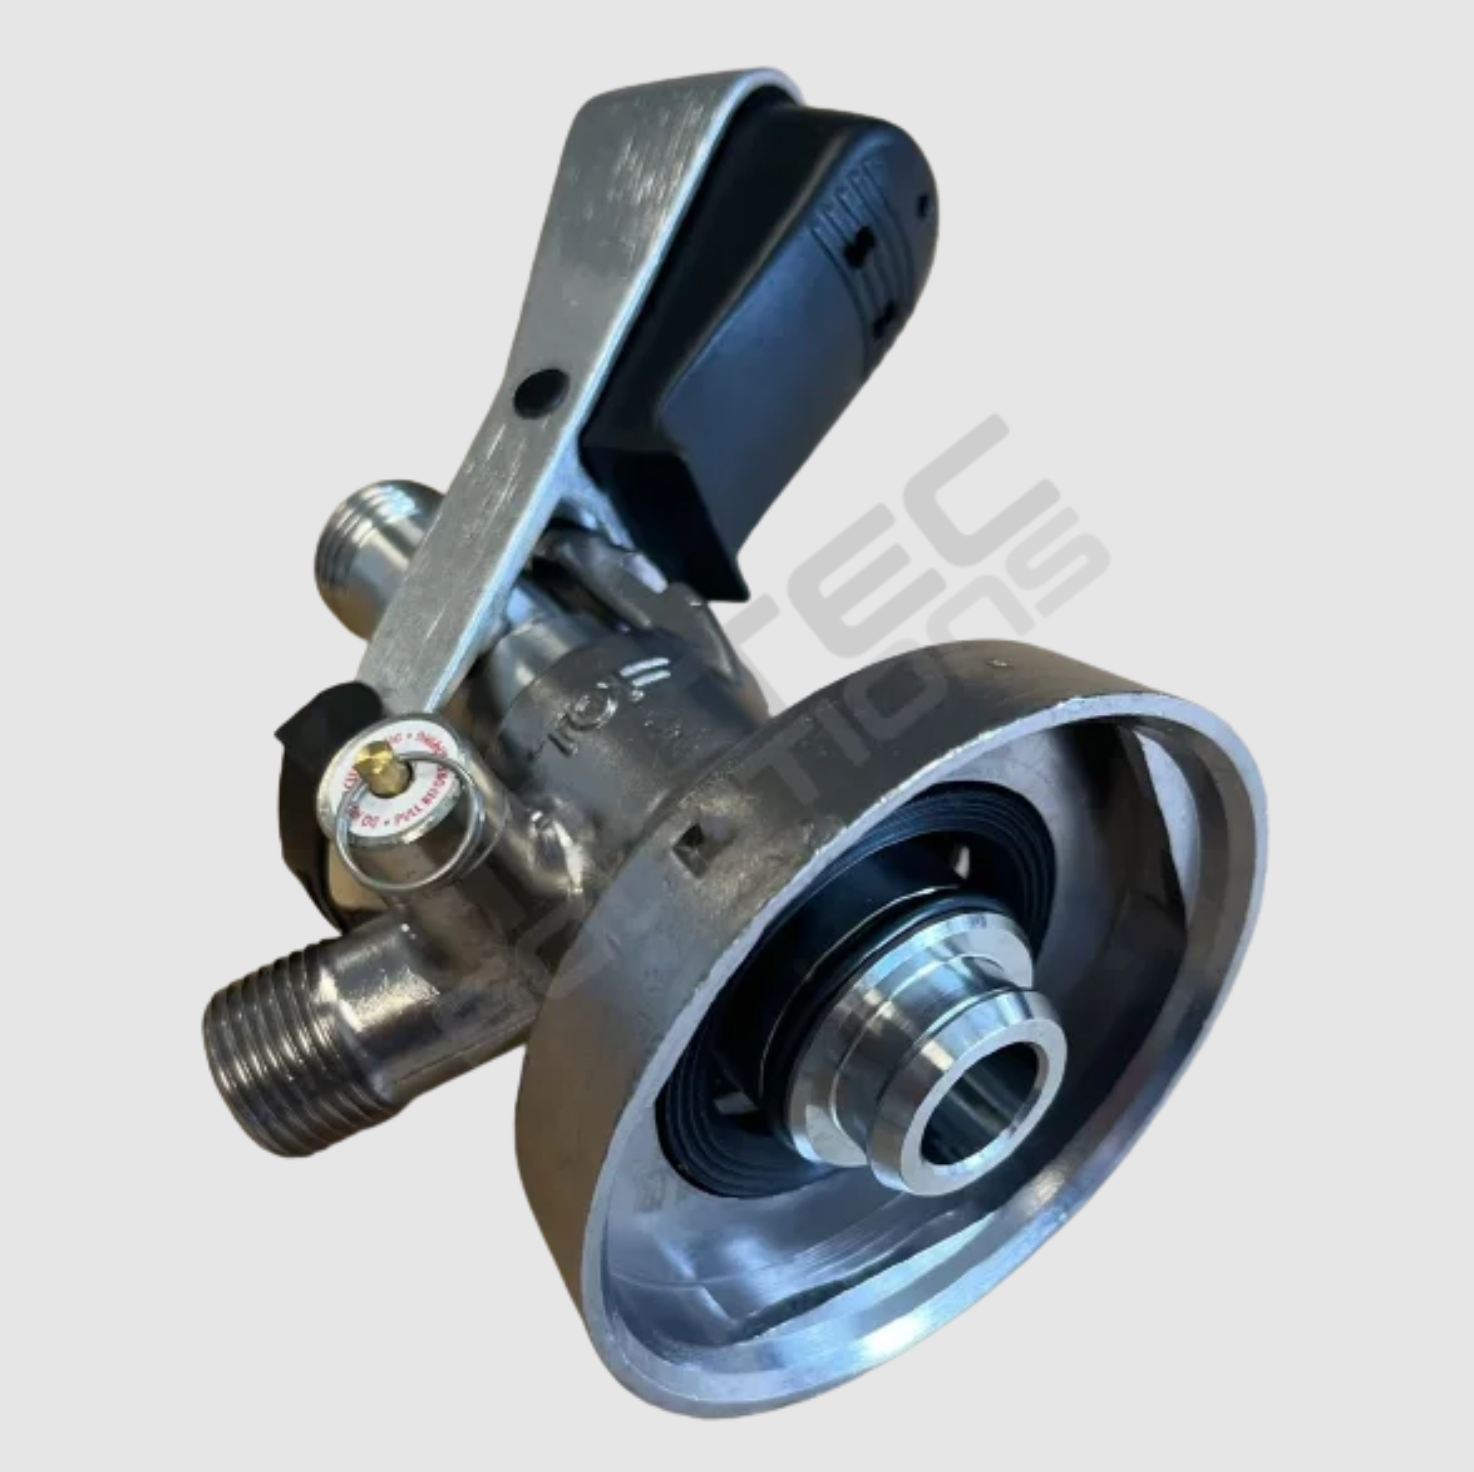
\includegraphics[width=0.5\textwidth]{KeyKeg-kobling.png}
    \caption{KeyKeg-kobling}
\end{figure*}

\subsection{A-kobling}
A-koblingen er slide-on koblingen, som bruges til f.eks. Ørbek (Fynsk Forår), Kronenbourg (Blanc 1664), og mange tyske/belgiske øl. Vi bruger den ikke fast, men har masser af A-koblinger.
\begin{figure*}[h]
    \centering
    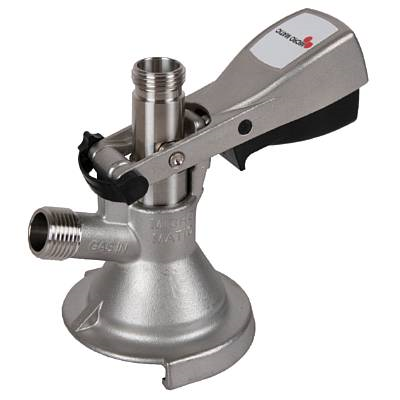
\includegraphics[width=0.5\textwidth]{A-kobling.png}
    \caption{A-kobling}
\end{figure*}


\end{document}
%%% Local Variables:
%%% mode: latex
%%% TeX-master: t
%%% End:

